\documentclass{beamer}
\usepackage[utf8]{inputenc}
\usetheme{Madrid}
\usecolortheme{default}
\usepackage{amsmath,amssymb,amsfonts,amsthm}
\usepackage{txfonts}
\usepackage{tkz-euclide}
\usepackage{listings}
\usepackage{adjustbox}
\usepackage{array}
\usepackage{tabularx}
\usepackage{gvv}
\usepackage{lmodern}
\usepackage{circuitikz}
\usepackage{tikz}
\usepackage{graphicx}

\setbeamertemplate{page number in head/foot}[totalframenumber]

\usepackage{tcolorbox}
\tcbuselibrary{minted,breakable,xparse,skins}



\definecolor{bg}{gray}{0.95}
\DeclareTCBListing{mintedbox}{O{}m!O{}}{%
  breakable=true,
  listing engine=minted,
  listing only,
  minted language=#2,
  minted style=default,
  minted options={%
    linenos,
    gobble=0,
    breaklines=true,
    breakafter=,,
    fontsize=\small,
    numbersep=8pt,
    #1},
  boxsep=0pt,
  left skip=0pt,
  right skip=0pt,
  left=25pt,
  right=0pt,
  top=3pt,
  bottom=3pt,
  arc=5pt,
  leftrule=0pt,
  rightrule=0pt,
  bottomrule=2pt,
  toprule=2pt,
  colback=bg,
  colframe=orange!70,
  enhanced,
  overlay={%
    \begin{tcbclipinterior}
    \fill[orange!20!white] (frame.south west) rectangle ([xshift=20pt]frame.north west);
    \end{tcbclipinterior}},
  #3,
}
\lstset{
    language=C,
    basicstyle=\ttfamily\small,
    keywordstyle=\color{blue},
    stringstyle=\color{orange},
    commentstyle=\color{green!60!black},
    numbers=left,
    numberstyle=\tiny\color{gray},
    breaklines=true,
    showstringspaces=false,
}
%------------------------------------------------------------
%This block of code defines the information to appear in the
%Title page
\title %optional
{4.8.13}

%\subtitle{A short story}

\author % (optional)
{BALU-ai25btech11017}



\begin{document}


\frame{\titlepage}
\begin{frame}{Question}
 Find the distance between the planes 
\begin{align}
\vec{r} \cdot (2\hat{i} - 3\hat{j} + 6\hat{k}) - 4 = 0
\quad \text{and} \quad
\vec{r} \cdot (6\hat{i} - 9\hat{j} + 18\hat{k}) + 30 = 0.
\end{align}
.\\ 
\end{frame}
\begin{frame}{Theoretical Solution}
Let us solve the given equation theoretically and then verify the solution computationally \\
According to the question, \\
Given two planes with direction vectors\\
\begin{align}
\vec{n_1}=\begin{myvec}{2\\-3\\6}\end{myvec}\
\vec{n_2}=\begin{myvec}{6\\-9\\18}\end{myvec}\
\end{align}
\begin{align}
    \vec{n_2}=3\vec{n_1}
\end{align}
so the are planes are parllel\\
Let us take a point in plane 1
\begin{align}
    \vec{A}=\begin{myvec}{2\\0\\0}\end{myvec}
\end{align}
\end{frame}
\begin{frame}{Theoretical Solution}
As planes are parllel distance from $\vec{A}$ to plane 2 is same as distance between planes\\
Let distance is k\\
\begin{align}
    k=\frac{(\vec{A}\vec{n_2}^T)+30}{\|\vec{n_2}\|}=2
\end{align}
\end{frame}
\begin{frame}[fragile]
    \frametitle{C Code}
    \begin{lstlisting}
#include <stdio.h>
#include <math.h>

int main(void) {
    /* Planes:
       Plane 1: 2x - 3y + 6z - 4 = 0    => a=2, b=-3, c=6, d1 = -4
       Plane 2: 6x - 9y + 18z + 30 = 0  => divide by 3:
                2x - 3y + 6z + 10 = 0  => d2 = 10
    */

    double a = 2.0, b = -3.0, c = 6.0;
    double d1 = -4.0, d2 = 10.0;

    double numerator = fabs(d2 - d1);              // |10 - (-4)| = 14
    double denominator = sqrt(a*a + b*b + c*c);    // sqrt(4 + 9 + 36) = sqrt(49) = 7
    double distance = numerator / denominator;     // 14 / 7 = 2

     \end{lstlisting}
\end{frame}
\begin{frame}[fragile]
    \frametitle{C Code }
    \begin{lstlisting}
      printf("Numerator |d2 - d1| = %.0f\n", numerator);
    printf("Denominator ||n|| = sqrt(a^2+b^2+c^2) = %.0f\n", denominator);
    printf("Distance between the planes = %.0f\n", distance);

    return 0;
}
\end{lstlisting}
\end{frame}
\begin{frame}[fragile]
    \frametitle{python code }
    \begin{lstlisting}
    import numpy as np
import matplotlib.pyplot as plt
from mpl_toolkits.mplot3d import Axes3D

# Define the planes:
# Plane 1: 2x - 3y + 6z - 4 = 0
# Plane 2: 6x - 9y + 18z + 30 = 0

# Normalize Plane 2 (divide by 3) → 2x - 3y + 6z + 10 = 0
# Now both planes are parallel with same normal vector n = (2, -3, 6)

# Grid for plotting
xx, yy = np.meshgrid(np.linspace(-10, 10, 20), np.linspace(-10, 10, 20))

# Plane 1: solve for z
zz1 = (4 - 2*xx + 3*yy) / 6






    \end{lstlisting}
\end{frame}
\begin{frame}[fragile]
    \frametitle{python code }
    \begin{lstlisting}
# Plane 2: solve for z
zz2 = (-10 - 2*xx + 3*yy) / 6

# Create 3D figure
fig = plt.figure(figsize=(10, 7))
ax = fig.add_subplot(111, projection='3d')

# Plot the planes
ax.plot_surface(xx, yy, zz1, alpha=0.5, color='blue', rstride=100, cstride=100, label='Plane 1')
ax.plot_surface(xx, yy, zz2, alpha=0.5, color='red', rstride=100, cstride=100, label='Plane 2')

# Normal vector
n = np.array([2, -3, 6])

# Pick a point on Plane 1 (let y=z=0, solve for x)
x0 = (4)/2  # when y=z=0
P1 = np.array([x0, 0, 0])
\end{lstlisting}
\end{frame}
\begin{frame}[fragile]
    \frametitle{python code }
    \begin{lstlisting}
# Distance formula: |d2 - d1| / ||n||
d1 = -4
d2 = 10
distance = abs(d2 - d1) / np.linalg.norm(n)

# Direction of normal vector (unit)
n_unit = n / np.linalg.norm(n)

# Point on Plane 2 along the normal
P2 = P1 + distance * n_unit

# Plot the connecting line (shortest distance)
ax.plot([P1[0], P2[0]], [P1[1], P2[1]], [P1[2], P2[2]], 'k--', linewidth=2)

# Mark points
ax.scatter(*P1, color='blue', s=50)
ax.scatter(*P2, color='red', s=50)
    \end{lstlisting}
\end{frame}
\begin{frame}[fragile]
    \frametitle{python code }
    \begin{lstlisting}
# Labels
ax.set_xlabel('X-axis')
ax.set_ylabel('Y-axis')
ax.set_zlabel('Z-axis')
ax.set_title(f"Distance between planes = {distance:.2f}")

# Save figure
plt.savefig("planes_distance.png", dpi=300)
plt.show()

    \end{lstlisting}
\end{frame}
\begin{frame}{Plot}
    \centering
    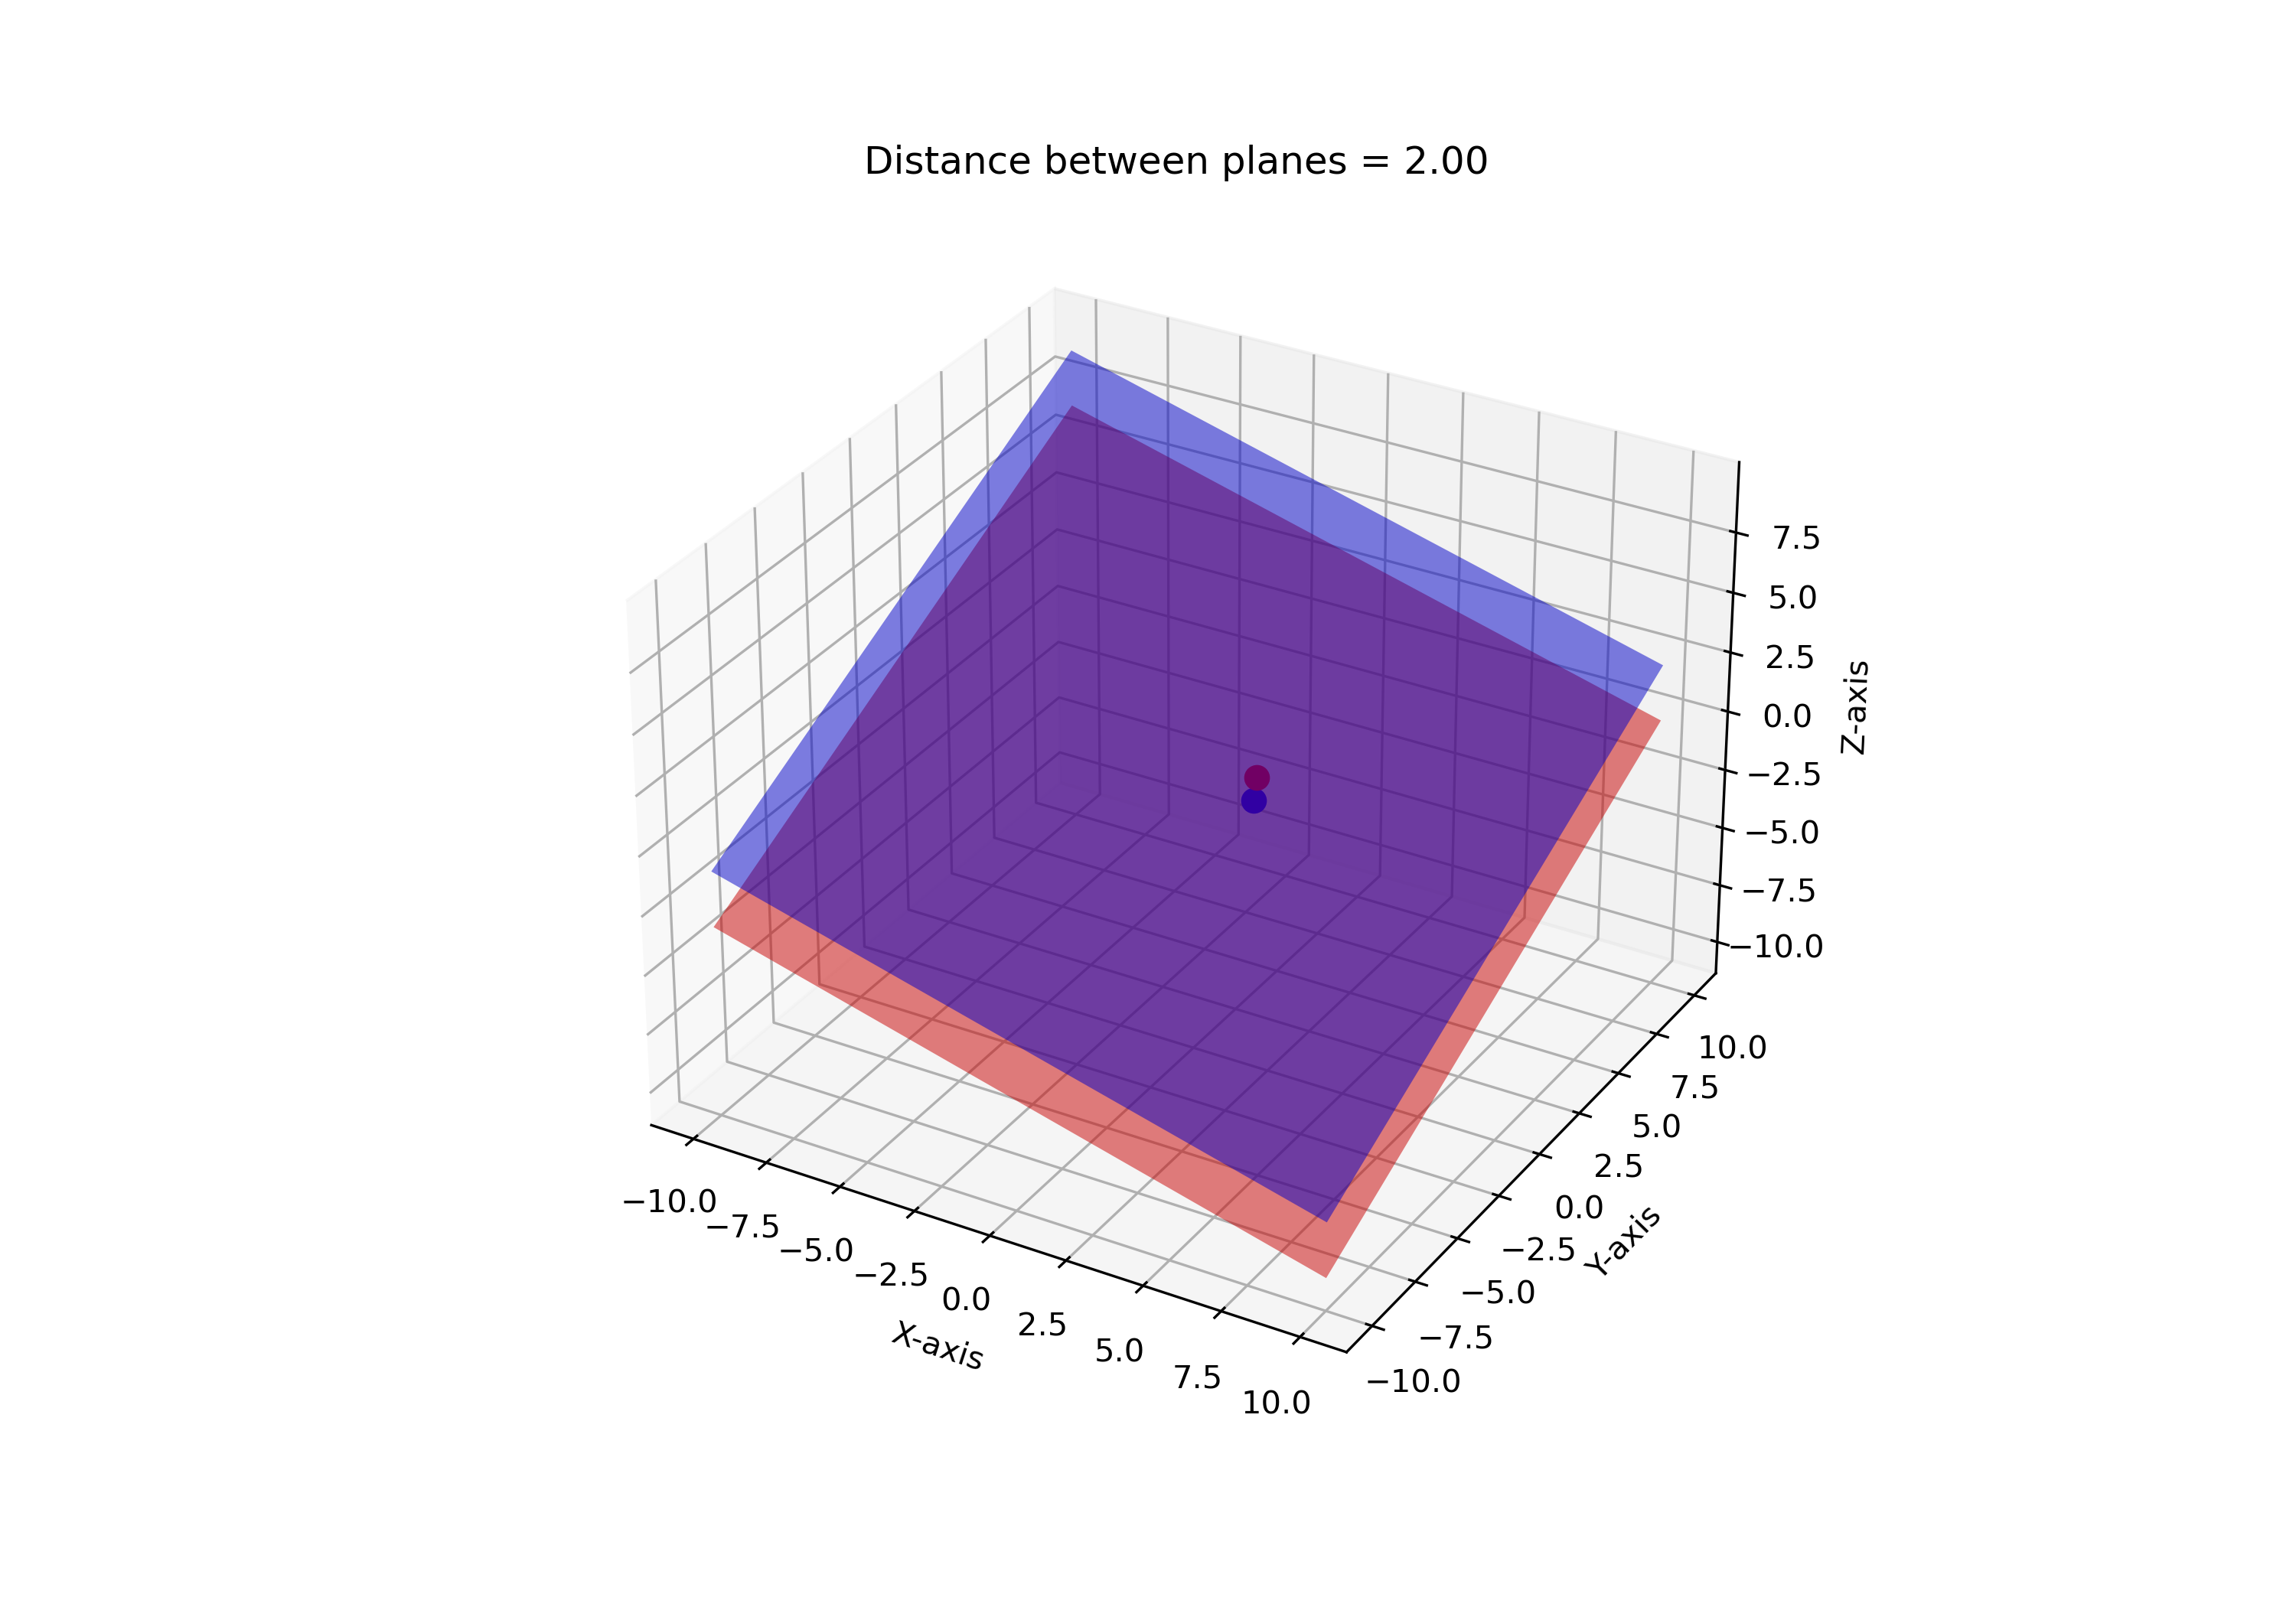
\includegraphics[width=\columnwidth, height=0.8\textheight, keepaspectratio]{figs/planes_distance.png}     
\end{frame}

\end{document}